%%%%%%%%%%%%%%%%%%%%%%%%%%%%%%%%%%%%%%%%%%%%%%%%%%%%%%%%%%%%%%%%
\begin{frame}[fragile]
\frametitle{\# 228: Doing Good}


 \begin{center}

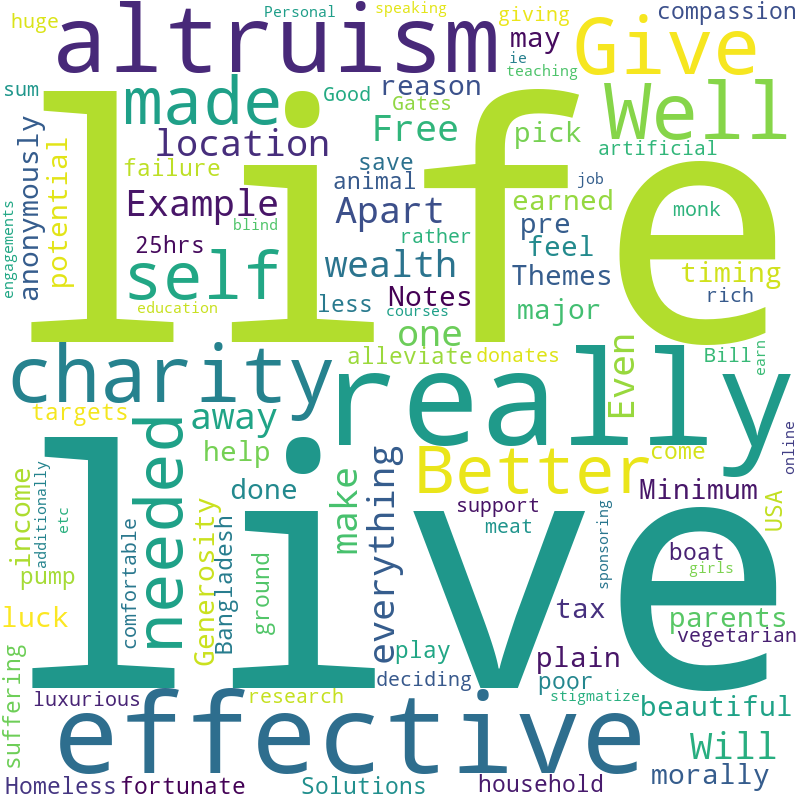
\includegraphics[width=0.6\linewidth,keepaspectratio]{images/Review_Podcast_MakingSene_228_DoingGood}
\end{center}

\end{frame}

%%%%%%%%%%%%%%%%%%%%%%%%%%%%%%%%%%%%%%%%%%%%%%%%%%%%%%%%%%%%%%%%
\begin{frame}[fragile]
\frametitle{\# 228: Doing Good}

 A Conversation with William MacAskill

% \begin{columns}[T] % align columns
% \begin{column}{.48\linewidth}
\begin{itemize}
\item Themes: Generosity, effective altruism.
\item Minimum 10\% of pre-tax income to most effective charity ("Give-Well")
\item  Better if done anonymously? Not really!! Taking public pledge.
\item  Altruism needed? Be self-made?
\item  You didn't pick location, parents, timing and plain luck. So, not really "self"-made. Like Will in Free-Will may not be really be Free.
\item  Even if you feel you have earned it, why not help? Have compassion for less fortunate.
% \end{itemize}
% \end{column}%
% \hfill%
% \begin{column}{.48\linewidth}
	% \begin{itemize}
	\end{itemize}
% \end{column}%
% \end{columns}

\end{frame}

%%%%%%%%%%%%%%%%%%%%%%%%%%%%%%%%%%%%%%%%%%%%%%%%%%%%%%%%%%%%%%%%
\begin{frame}[fragile]
\frametitle{\# 228: Doing Good}

% \begin{columns}[T] % align columns
% \begin{column}{.48\linewidth}
\begin{itemize}
% \end{itemize}
% \end{column}%
% \hfill%
% \begin{column}{.48\linewidth}
	% \begin{itemize}
	\item Solutions should come from the ground. Example of failure: 25hrs on play-pump needed for one household.
	\item  What are targets for charity? Homeless in USA or poor in Bangladesh?
	\item  Make life boat better, to save more.
	\item  To alleviate animal suffering: be vegetarian, support artificial meat research
	\item  Good example: Bill Gates lives a luxurious life and donates huge sum as well, rather than deciding to live like a monk while giving away everything else. Even other rich are comfortable doing same. Don't stigmatize wealth.
	\end{itemize}
% \end{column}%
% \end{columns}

[Personal: Apart from sponsoring blind girls education, additionally, I give away everything I earn apart from my job, ie from my speaking engagements, online courses, teaching, etc.]
\end{frame}

% %%%%%%%%%%%%%%%%%%%%%%%%%%%%%%%%%%%%%%%%%%%%%%%%%%%%%%%%%%%%%%%%
% \begin{frame}[fragile]
% \frametitle{Prelude}

% \begin{columns}[T] % align columns
% \begin{column}{.48\textwidth}
% \begin{itemize}
% \item Mind is divided into 4 sections
	% \begin{itemize}
	% \item Section 1 : Brain
	% \item Section 2 a: RAS
	% \item Section 2 b: CCS
	% \item Section 3 : Extra Sensory Perceptions
	% \item Section 4 : Soul (atman)
	% \end{itemize}
% \item RAS:
% \item CCS: Critical Certain Stage
% \item Lower Dimension: 1, 2a
% \item Higher Dimension: 2b, 3, 4
% \end{itemize}
% \end{column}%
% \hfill%
% \begin{column}{.48\textwidth}
 % \begin{center}
% \includegraphics[width=0.9\linewidth,keepaspectratio]{images/zenyoga1}
% \end{center}

% \end{column}%
% \end{columns}
% \end{frame}

% %%%%%%%%%%%%%%%%%%%%%%%%%%%%%%%%%%%%%%%%%%%%%%%%%%%%%%%%%%%%%%%%
% \begin{frame}[fragile]
% \frametitle{Section 2a}
% \begin{itemize}
% \item Intercepts flow from physical body, senses.
% \item Adjusts/tones-down/accentuates and sends to thalamus to cortex for decision making.
% \item Thus body can report bodily disorders to brain directly without consulting conscious mind.
% \item This covers all unconscious/autonomous functions.
% \end{itemize}
% \end{frame}

% %%%%%%%%%%%%%%%%%%%%%%%%%%%%%%%%%%%%%%%%%%%%%%%%%%%%%%%%%%%%%%%%
% \begin{frame}[fragile]
% \frametitle{Section 2b}
% Concentration, Meditation, Intuition.

 % \begin{center}
% \includegraphics[width=0.35\linewidth,keepaspectratio]{images/zenyoga2}
% \end{center}

% Goal: Cross the divide (no-mans-land) and go to CCS and further.

% \end{frame}
